\chapter{Design}

In this section we are going to see the Architectural design of the MPLS Opportunistic Security and the motivation behind the design. We will see each and every technologies used in the design too.

\section{Three Pillars of Security}

\subsection{Confidentiality}

Confidentiality in MPLS networks
deals with a number of areas, including confidentiality of
Label Information Base (LIB) and confidentiality of
traffic passing through the system's infrastructure. The exposure
of LIB can lead to a number of security problems if LSR
accepts labeled packets from hosts outside the core. To
avoid brute-force enumeration of label values, it
must be ensured that no labeled packets are accepted
from outside the MPLS infrastructure. Unlike common VPN technology (IPSec or SSL VPNs) MPLS VPNs do not provide any confidentiality about the traffic data.
Moreover, MPLS network architecture does
not provide header or payload encryption. The main purpose of MPLS technology is to provide high speed
packet delivery and this is the reason why it doesn't provide any encryption mechanisms. In initial days, security features in MPLS network were given a least importance since most of the emphasis was given to speed related features. Due to recent market demands and researches of the security features, now the security considerations in MPLS are studied thoroughly. In typical IP networks,
every router in the network analyzes IP
packets headers, to classify, and to process all the
packets  which passes through it. This eventually will add more
overhead and delay in the network. In
MPLS network, only two routers (the ingress and
egress routers) are responsible for this activity. Core or
LSR routers in MPLS network will only forward
packets based on labels transmitted through a preestablished
LSP. The use of encryption to provide
privacy of data requires the core MPLS routers to
analyze and process packets’ header, which will result
in reducing the performance of MPLS network.

\subsection{Integrity}

As we know that ISP mostly will not employ any system to protect the data and traffic flow between the MPLS Routers as plain text. If an attacker get access inside the MPLS Network, he/she can modify the packet for his/her benefits. The MPLS Network should be protected in such a way that none of the nodes of the Network is exposed for any kind of packet modification.

\subsection{Availability}

blocking or not accepting Label
Distribution protocol and RSVP protocol update packets from an unauthorised client is very important. Accepting such updates can even lead to LSP removals and affect the availability. Sometimes accepting LDP updates from a malicious client or creating LDP session with a malicious peer can harm the network in such a way that the traffic can get redirected. Hence Authenticating an LDP peer is very important. 


\section{Opportunistic security (OS)}

Most of the time the internet service provider send the data through their network as they have to meet the Service Level Agreements with the customers. The SLA are mainly with respect to the throughput and latency. If they take the responsibility of encryption and decryption hop-by-hop, for sure they won’t be able to meet the SLAs. Hence they provide these security requirements end to end instead of hop-by-hop and users has to trust the service provider. At times even the Service Provider will compromise on the security of data when meeting the SLA is challenge, example peak traffic time. Service Providers has to implement many tools to assure the data security and administrating various features and protocols and its maintenance such as Key validation, procuring license etc are a challenge and that is another reason why the Service Providers often offload these responsibility to the end user systems. 


Nowadays most of the web services use VPN devices Public Key Infrastructure (PKI) for authenticating peers.  IPSec, SSL, and TLS is widely relied on PKI. In order to do so, one has to maintain a licensed Certificate Authority and it’s a challenge. Trusting a certificate authority is again a challenge. Many service provider will have issues on trust with the Certificate Authority and this might lead to the disagreement between users who are trying to connect and sometimes the service has to compromise on peer authentication and when the authentication is an optional service, then the traffic will be either send in plain text without any security or in cipher text with some security and most of the case the security provided are either ‘NULL’ or minimum and rarely with complete.

In Opportunistic Security, the baseline communication is in plain text and with encryption and authentication by negotiation between peers when available and the negotiated algorithms and techniques are used for encryption and authentication. If authentication is not available, then at least encrypt the data and if both are not available, send the data in plain text. Opportunistic Security is not an alternative for authenticated, encrypted data transfer when tools for such operation is already in place. It is only used when encrypted and authenticated data communication is needed otherwise go for plain text.

\subsection{OS in MPLS} 

As we discussed above the basic requirement of MPLS Opportunistic Security\cite{__2017} is encrypt the data between MPLS Routers with the a key both the routers are negotiated with. The has to be derived by a diffie-hellman key exchange. The generated session key after the Diffie-Hellmans key exchange is used for the packet encryption. The Algorithm to be used for encryption should be any flavours of AES and it should use in GCM mode for the payload authentication. The key derived should be according to the algorithm going to use which should be negotiated by exchanging TLVs.  The key length will change from 128 bit to 256 bits according to the algorithm of choice.


\subsubsection{Diffie-Hellman Key Exchange} 

Diffie-Hellman Key Exchange(DH)\cite{just}\cite{rescorla_1999} is a way of generating a share key by sharing private values computed with public values by 2 peers. Here I am going to explain how the shared key is generated.
Let’s take  the example of participants  Alice and Bob (Name is just for a reference). Let Alice and Bob choose a shared base and shared prime. Let Alice and Bob choose the shared base (g) = 5 and shared prime (p) = 23. At the same time Alice and Bob should have their private values called secrets. Let Alice choose the secret (a) = 6 and Bob secret (b)= 15. Now Alice will send a number  to Bob which is shared base to the power of Alice’s secret modulus shared prime( A = g\^a mod p) and Bob send a number to Alice which is shared base to the power of Bob’s secret modulus shared prime( B = g\^b mod p). Now Alice can calculate the shared secrete by computing  received number (B) to the power of Alice secret then modulus with shared prime ( Alice Shared Secret = (B\^a mod p) )and Bob can calculate the shared secret by computing received number (A) to the power of Bob secret then modulus with shared prime ( Bob Shared Secret = (A\^b mod p) ). In the above example the shared secret will be 2.

\subsubsection{Advanced Encryption Standard (AES) - Galois/Counter Mode (GCM)}



Advanced Encryption Standard\cite{robertazzi_2011}\cite{denis_johnson_2007} is an encryption algorithm designed and developed by US National Institute and Technology in 2001. It,s a blockcipher algorithm and developed by Vincent Rijmen and Joan Daemon. The algorithm is capable of handling block encryption with key sizes 128, 192 and 256 bits. It’s expected that AES can serve next 30 years and its freely usable in all devices. AES-GSM is such an algorithm which can provide data confidentiality (encryption), data Integrity and authentication. GCM is very efficient in parallel processing. In MPLS Opportunistic Security, authentication, encryption and data Integrity is served using AESGCM-128 and the key is derived using Diffie Hellmans Key exchange.

\subsection{MPLS Packet Encryption} 

In MPLS OS the MPLS packet is encrypted using AES-128-GCM algorithm and the key and initialisation vector are derived by the Diffie-Hellman Key exchange by the 2 participating end to end or hop by hop Label Switched Routers, it can be Provider edge routers or Provider Routers. A special purpose label called MPLS Encryption Label (MEL) will be added to the encrypted MPLS packet and thus we can identify the encryption state. The S flag (Bottom of Stack) of the MEL is set to one and the MEL is followed by a a 4 byte header of the Pseudowire control word (Ethernet PWCW).

The nonce used in the encryption algorithm is derived from the HMAC based Key Derivation Function called HKDF and this nonce will be incremented by on for each encrypted packet and the same nonce used for successful deception. The control word (CW) carries the lower order 16 bits of the nonce which is used to identify packet drop at the LSR as well as it helps to process the deception in the same order of encryption. 

The CW is a 4 byte header with a control field data and a sequence number. The lower order 16 bits of the nonce is send as sequence number in the CW header. This sequence number is used for identifying any packet drop or mismatch in the IV packet counter. If the sequence number received through CW header is matching the receiving LSRs counter, then packet will be decrypted. If the packet drop is more than 65535 packets , then the receiving side Router will stop further decryption and alert the encrypting router about the same. The additional authentication tag generated by the AES-GCM algorithm will be attached with the cipher data which makes the encrypted packet slightly bigger than the original packet. The authentication tag is used for authenticating the data after the decryption.


\begin{figure}
       \centering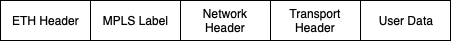
\includegraphics[width=\textwidth]{Final/MPLS.png}
       \caption{MPLS Packet}
       \label{fig:compbest}
\end{figure}


n Normal MPLS Packet, there will be a MPLS Label with bottom-of-stack flag set to 1 pushed on top of the payload. There can be underlying Labels too but with the bottom-of-stack(S) flag set to 
0. The Ethernet header is pushed below all the MPLS Labels and Layer3 Header, Layer 4 header and user data is pushed above all the labels.

\begin{figure}
       \centering
\includegraphics[width=\textwidth]{Final/MPLSOS Packet.jpg}
       \caption{MPLS OS Packet}
       \label{fig:compbest}
\end{figure}


 In the proposed MPLS OS packet, Ethernet Header and top MPLS label remain same. The top MPLS label is then follow another special purpose label with value 15 and bottom-of-stack 0. The special purpose label is then follow MEL followed by CW. Layer3 header, Layer 4 header and user data is encrypted. 

MEL (MPLS Encryption Label) : MEL is like normal MPLS Header, but with the labels from the reserved experimental range (240-255). This label assignment makes it different from normal MPLS Header.Traffic Control (TC) bit is set to the value of the top MPLS Label. S bit is set to 1.

Label 
This label is a special purpose label and so far no special purpose label is allocated by IANA. Hence we have to choose one of the reserved experimental labels from range 240-255.

Traffic Class (TC)
TC is a 3 bit field in the MEL Header. TC is basically used for QoS and ECN. The TC Value should filled the same as the primary outer MPLS Header which is not encrypted.

Bottom of Stack (S)
As MEL is in the bottom of the MPLS Stack, the flag S of the MEL Header should be always set to 1. 

\subsubsection{Control Word (CW)}

\begin{figure}
       \centering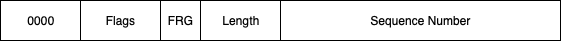
\includegraphics[width=\textwidth]{Final/CW.png}
       \caption{CW Header}
       \label{fig:compbest}
\end{figure}


Control Word (CW) is a 4 byte header. 1st 16 bits of CW is for setting the control word data and the last 16 bits are for sequence number which is nothing but the lower order 16 bits of the nonce. Whenever a packet received at LSR, it will check the underlying protocol of the packet. If the packet is an IP packet, then it will forward by normal routing if so configured. If it is an MPLS packet, it will PUSH/POP the label based on the destination. If the packet have CW and MEL, then the LSR understand that its an encrypted packet and cannot check the underlying protocol for packet forwarding\\

\subsubsection{0000}
The first 4 bits of the CW header is set to 0000 to indicate its a MPLS payload.\\

\subsubsection{Flags} 
Flags is a 4 bit field in the CW Header which contains the session key-id, so that the participants can identify the algorithms and key to be used.\\


\subsubsection{FRG} 
This is a 1 bit field in the CW header and its set to 0 always as MPLS doesn’t support fragmentation\\ 

\subsubsection{Length}
Value of Length should be set to 0 and receiving LSR can ignore this flag.\\

\subsubsection{Sequence Number}
This field contains the low-order 16 bits of the nonce that is currently being used for the agreed encryption parameters. It is indicative of the counter used in the AEAD- AES-GCM encryption which the receiving LSR can use to check it its counter is correct and if it can go ahead with the decryption.\\

Anything from the layer 3 to layer 7 of the packet is encrypted\\

\section{Technologies Involved} 

OpenVswitch, Mininet, OpenFlow, Linux Crypto APIs, Kernel forwarding are the important technologies used in the project. We can see each of them in detail.


\subsection{Mininet} 


Mininet\cite{team}\cite{de2014using} is an emulated network orchestration system. We can emulate Linux hosts, routers, and switches using simple commands and connect them whatever the way and order we want. Mininet links all the emulated hosts and network devices to the same Linux kernel. It is using lightweight virtualisation to make simple and complete network topology which is running the same kernel. The host emulated by Mininet behave exactly the same way the real host behaves except the fact that, there is no real hardware. We can create ssh sessions to all the hosts and switches using the command xterm<space>hostname in the Mininet command line interface.  We can send packets from hosts to host which can be monitored using tcpdump or Wireshark and the packet captured will be absolutely equivalent to the packet captured from a real networking hardware. We can measure speed of the links using tools like Iperf and the link speed between the hosts and routers can be configured or changed using Mininet commands. In short, all the emulated networking devices by Mininet behaves and resembles the same way we expect a hardware product should be behaving.
 
\begin{figure}
       \centering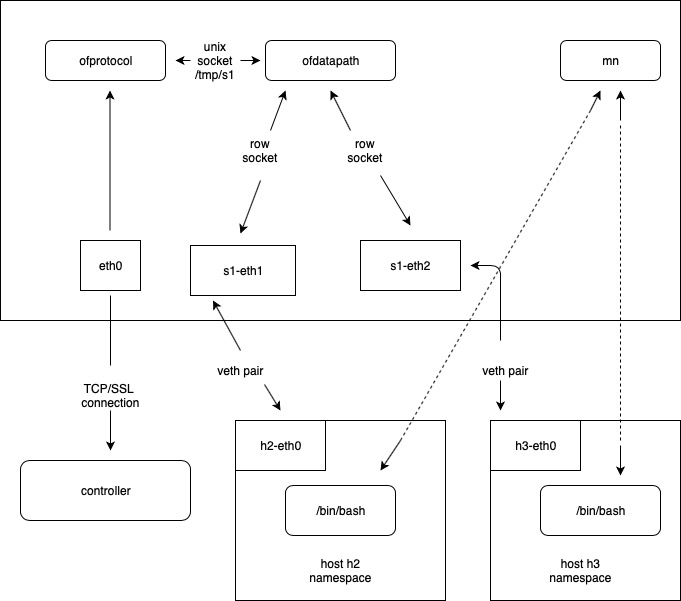
\includegraphics[width=\textwidth]{Final/mininet architecture.jpg}
       \caption{Mininet Architecture}
       \label{fig:compbest}
\end{figure}

\subsection{OpenVSwitch (OVS)} 


OpenVSwitch\cite{openvswitch}\cite{OVS} is an open source multilayer software with Apache 2 license. OpenVSwitch is designed for functioning as a virtual switch in both virtual environment and hardware. The OpenVSwitch code (OVS) can be configured and installed in any linux operating system. It supports most of the linux based virtualization techniques such as Virtual box, KVM, Xen/XenServer etc. The OVS code is written in platform independent C and can be used and ported to other environments. Basically OpenVSwitch is designed for automating large-scale network topology using programmatic extension. OpenVSwitch support standard management interfaces such as Flow, IPFIX, 802.1ag, NetFlow etc. As of now OpenVSwitch cannot run on hypervisors like VMware ESXi and Microsoft Hyper-V, but the development is going on to support them in near future. The 2 major components of OpenVSwitch are  ovs-vswitchd and datapath kernel module. ovs-vswitchd is a daemon which is running in the userspace. Then ovs-vswitchd will not be the same in each operating system but identical in the service. The datapath kernel module functions in the kernel level. The best part is that, we can modify the datapath kernel module and compile and load on the operating system kernel without changing the operating systems kernel. \\

\begin{figure}
       \centering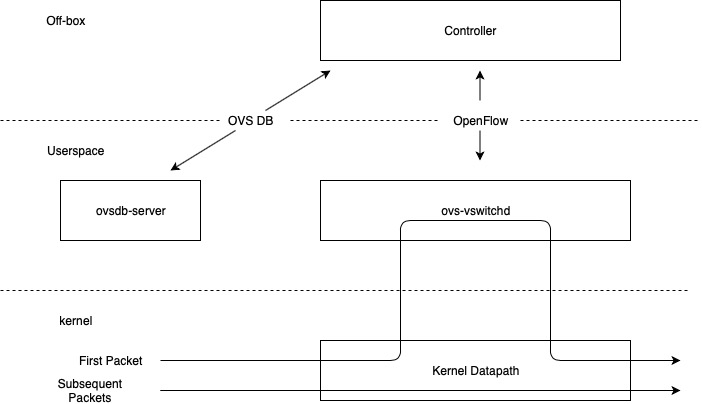
\includegraphics[width=\textwidth]{Final/OVS Architecture-2.jpg}
       \caption{OVS Architecture}
       \label{fig:compbest}
\end{figure}

The first packet entering the NIC is taken into the datapath kernel module and there are 2 possible actions to perform on the packet. If there is any set of actions and logic instructed by the ovs-vswitchd, then perform the logic and forward the packet. If there is no logic instructed, then pass the packet to ovs-vswitchd and wait for the instruction. The subsequent packets belongs to the same flow will be forwarded using the flow logic applied to the first packet.



\subsubsection{Kernel Forwarding} 

All the packets from NIC is taken into the kernel. The daemon ovs-vswitchd is the one instruct the kernel what actions need to be performed on the packet. The actions can be encapsulation, decapsulation, reroute, sampling, drop etc. The kernel datapath will perform these actions on the packet and forward the packets. Generally the ovs-vswitchd actions are instrucrted by the user (administrator) based on the flow. Flow is nothing but packets with same source address, same destination address, same source port, same destination port and same protocol. OVS Actions can be applied even the flows are partially matching. Once the first packet forwarded out with the logic/action from the ovs-vswitchd, the kernel datapath will store the instructions in its local cache and perform the same action if the subsequent packets are eligible for the same actions. If the new packet doesn’t match with the flow marked in the cache, it will treat like the first packet and taken into Userpace and then ovs-vswitchd.


\subsubsection{Userspace Forwarding} 

As we seen in the kernel forwarding, kernel datapath maintain the local cache with the instructions received from ovs-vswitchd for the flows which kernel forwarded to  ovs-vswitchd. If there is no cache available for the incoming flow, then the packet will be taken into ovs-vswitchd which is running in userspace. OpenVSwitch maintain a flow table which is generated based on the cache and this table will say what actions to be performed on the packet. As OpenVSwitch used as SDN switch, the OVS controller and OVS Switch talk to each other using OpenFlow. The user can instruct the OVS controller the actions to be performed in each switch then  OVS Controller instruct the  ovs-vswitchd and finally ovs-vswitchd instructs the datapath kernel module. 

 
\subsection{OpenFlow} 

OpenFLow\cite{2016} is a protocol used for communicating between SDN controller and SDN Switches. As we know that the control plane of the SND Lies in the controller and the controller instruct the data planes (Switches and Routers) what are the actions need to be performed on the incoming packet. This control message exchange between SDN Controller and other nodes usually using open flow protocol. OpenFlow is more like an instruction set similar to x86 instruction set and it provides an open interface to the nodes such as routers and switches. The SDN nodes will have flow tables which is about what are the actions to be performed to an incoming traffic from a particular interface with a particular flow. The open protocol of  OpenFLow is used to program the flow table. The instructions are in the form of flow entries in the flow table. As the SDN controller is remotely accessible from remote locations, researchers and administrators can use open flow to control open flow tables of connected switches and routers and thus control the packet forwarding. \\
 
\subsection{Architecture of Experiment}

The Network topology is emulated using Mininet and packets are processed using openvswitch. the emulated switches will be running with OVSK. Openvswitch can be used in docker and containers too but each docker will have its own overhead and it will affect the network performance. Mininet is very fast to build up the network and tear down the network and hence Mininet is the best choice to demonstrate the MPLS OS using OVS. By default OpenVSwitch will be installed along with Mininet and the Installed openvswitch will be replaced by the modified OpenVSwitch separately installed. Mininet require a controller, a kernel and \\

\begin{figure}
       \centering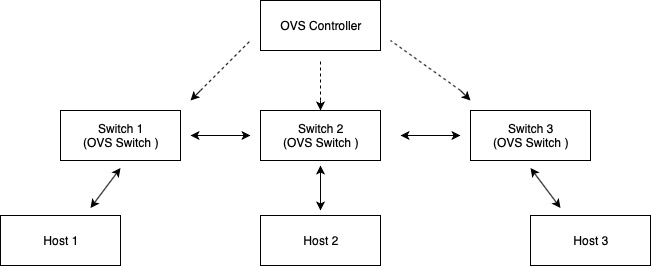
\includegraphics[width=\textwidth]{Final/Experiment Topology.jpg}
       \caption{Experiment Topology}
       \label{fig:compbest}
\end{figure}

In the experiment topology, we will be creating 3 switches (S1, S2 and S3) connected linearly. Each switch is connected 1 host. Switch S1 have 2 interfaces s1-eth1 and s1-eth2. S1-eth1 is connected to Host 1 and s1-eth2 is connected to s2-eth2 of Switch S2. S2-eth1 of switch S2 is connected to Host 2 and s2-eth3 is connected to s3-eth2 of Switch S3. Interface s3-eth1 of S3 is connected to Host 3.
The controller is connected to all the switches and it will update the flow rules in all the switches.\\

The hop by hop behaviour of normal MPLS traffic in our test topology without MPLS OS is as follows:\\

Step 1 : Host 1 initiated an ICMP Ping to Host H3\\
Step 2:  H1 check in its arp table for a the destination MAC address.\\
Step 3: As its the first packet and there is no arp entries for the corresponding destination (Host 3), Host 1 will send an arp request to Host 3.\\
Step 4: Arp request packet will reach Switch 1 ethernet 1 interface and Switch 1 will send the packet out of ethernet 2 interface.\\
Step 5: Arp request packet will reach Switch 2 ethernet 2 interface and Switch 2 will send the packet out of ethernet 3 interface.\\
Step 6: Arp request packet will reach Switch 3 ethernet 2 interface and Switch 3 will send the packet out of ethernet 1 interface.\\
Step 7: H3 will receive the Arp request packet and respond by an ARP reply and it will take the reverse path of ARP Request.\\
Step 8: H1 will send the ICMP packet to the S1 through ethernet 1 ethernet interface.\\
Step 9: S1 will receive the ICMP packet from ethernet 1 interface. S1 will push the MPLS label send out of ethernet 2 interface.\\
Step 10: Switch 2 receive the MPLS packet from ethernet 2 interface and it will send the packet out of ethernet 3 interface.\\
Step 11: Switch 3 receive the MPLS packet from ethernet 2 interface and it will pop the MPLS Label out and send the ICMP packet out of ethernet 1 interface.\\
Step 12:  H3 will receive the ICMP packet from ethernet 1 interface and it will reply back to H1. The reply packet will take the reverse path of incoming ICMP packet, S3 will push the label and S1 will pop the label.\\

The hop by hop behaviour of normal MPLS traffic in our test topology with MPLS OS is as follows:\\

Step 1 : Host 1 initiated an ICMP Ping to Host H3\\
Step 2:  H1 check in its arp table for a the destination MAC address.\\
Step 3: As its the first packet and there is no arp entries for the corresponding destination (Host 3), Host 1 will send an arp request to Host 3.\\
Step 4: Arp request packet will reach Switch 1 ethernet 1 interface and Switch 1 will send the packet out of ethernet 2 interface.\\
Step 5: Arp request packet will reach Switch 2 ethernet 2 interface and Switch 2 will send the packet out of ethernet 3 interface.\\
Step 6: Arp request packet will reach Switch 3 ethernet 2 interface and Switch 3 will send the packet out of ethernet 1 interface.\\
Step 7: H3 will receive the Arp request packet and respond by an ARP reply and it will take the reverse path of ARP Request.\\
Step 8: H1 will send the ICMP packet to the S1 through ethernet 1 ethernet interface.\\

Step 9: S1 will receive the ICMP packet from ethernet 1 interface. S1 will check for the generated shared secret key for encryption.\\
Step 10:As there on key available, S1 will initiate a DH key exchange with S3. S1 will use the incoming ICMP traffic for the DH exchange. S1 will push the MPLS Label and add the MPLS TLV          between MAC header and MPLS header. This TLV will have the information such as DH group, Encryption algorithm, DH Key etc.\\
Step 11: Switch 2 receive the MPLS packet from ethernet 2 interface and it will send the packet out of ethernet 3 interface.\\
Step 12: Switch 3 receive the MPLS packet from ethernet 2 interface and it will pop the MPLS Label and MPLS TLV out and send the ICMP packet out of ethernet 1 interface.Switch 3 will get the DH Key of the S1 from the TLV and it will calculate the shared secret key for encryption and decryption.\\
Step 13: H3 will reply to the ICMP request and the request will reach Switch 3 ethernet 1.\\
Step 14: S3 will push the MPLS Label and add the MPLS TLV between MAC header and MPLS header. This packet will follow the reverse path of packet from H1 to H3.\\
Step 15: When the reverse packet arrived at S1, it will pop the MPLS Label and the MPLS TLV and the send the plain ICMP too H1.\\
Step 16: Switch S1 will get the DH Key of the S3 from the TLV and it will calculate the shared secret key for encryption and decryption.\\
Step 17: Second ICMP Ping packet from H1 to H3 arrived at S1 at ethernet 1 interface.\\
Step 18: S1 will encrypt the payload using  AES-GCM encryption algorithm and the key used is generated in the previous steps. After encryption, a CW header will be pushed on top, then the MPLS Encryption label will be pushed on top. The normal MPLS Header will be pushed on top of the MEL and will send the packet out of ethernet 2 interface.\\
Step 19: Switch 2 receive the MPLS packet from ethernet 2 interface and it will send the packet out of ethernet 3 interface.\\
Step 20: Switch 3 receive the encrypted MPLS packet. It will pop the MPLS label, MEL label and CW header. S3 then decrypt the packet and send then plain ICMP Packet out of ethernet 1 to H3.\\
Step 21: ICMP reply from H3 to H1 will be encrypted at S3 and add MEL, CW Header and MPLS label and send to S1 and S1 will decrypt the packet and send to H1.\\

The Diffie-Hellman Key exchange is not fully integrated in this project work even though the participating switches are exchanging keys and generating shared secret. The MPLS TLV is not exactly same as the specifications since some fields in the TLV such as LSP ID is not available OVS as the labels are manually supplied .HKDF is not implemented in this project and The DH Key is send as an integer decimal in the TLV instead of string. The Generated shared key is used for encryption and decryption.  



